%!Mode:: "TeX:UTF-8"

\section{C++与C的区别}



\subsection{指针和引用}
没有null引用,引用不可重新赋值。

\subsection{struct和class}
不同的默认成员保护级别;不同的默认派生保护级别(class默认private继承);此外没有区别。

\subsection{type castsing与强制类型转换}
\verb|static_cast|等四种转型操作相对于C风格强制类型转换的优势:
1.容易辨识,不论是人工识别还是grep
2.各转型动作目标越窄化,编译器越可能诊断出错误的运用

\subsection{iostream相对于stdio}
1.类型安全;2.易扩展

类型安全代码指访问被授权可以访问的内存位置。例如,类型安全代码不能从其他对象的私有字段读取值。
它只从定义完善的允许方式访问类型才能读取。类型安全的代码具备定义良好的数据类型。

类型安全可以理解为归功于C++的封装与权限控制机制。

易扩展可以理解为归功于C++的重载、泛型等机制。

\subsection{宏调用与内联函数}
相比于内联函数,使用宏代码最大的缺点是容易出错,例如产生边际效应:
\begin{lstlisting}[language=C]
#define MAX(a, b) (a) > (b) ? (a) : (b) 
result = MAX(i, j) + 2;
\end{lstlisting}
这里加法优先级高于冒号,因此得不到预期结果,应该将整个宏定义括起来。
再比如\verb$result = MAX(i++, j); $也因为做不到\textbf{引用透明性}而易导致出错。

\begin{quotation}
表达式的引用透明性(Referential transparency,referential opacity)是指将表达式用其结果来替换,程序结果不变。
引用透明性是函数式编程(如Common Lisp, Haskell)的基础,只有做到了引用透明性,函数的结果才可被缓存。
用引用不透明来描述宏调用的缺陷不太合适, 除非理解为拿MAX(i++,j)和{MAX(i,j);i++}作比较。
\end{quotation}

此外,编译器不会对宏调用进行类型检查;宏定义也无法访问类中成员。

inline函数相对于普通函数的缺点包括:\\
可能造成代码体积膨胀,cache丢失;无法随程序库而升级,客户必须重编代码;调试器对inline束手无策。

\subsection{如何混编C和C++}
使用extern C防止Name Mangling;使用\verb$#ifdef __cplusplus$判断当前编译器。


%################################################################

\section{C++ 重要语法}


\subsection{引用与临时对象}
non-const引用形参只能对应non-const实参,且类型必须匹配。
const引用形参可以接受类型不匹配的变量和表达式,会导致生成临时对象。

返回引用与返回对象在正确性与效率上的区别:
\begin{enumerate}
  \item 对于多态对象,如果返回基类对象value,会导致对象切割(slicing),该对象不再具有多态行为
  \item 返回引用更高效
\end{enumerate}
但是,对于临时对象,不要返回引用。

C++的临时对象:
\begin{enumerate}
\item 函数调用时隐式类型转换时以求调用成功
\item 函数返回对象的时候
\end{enumerate}

返回值优化(Return value optimization,缩写为RVO)是C++的一项编译优化技术,取消了存放函数返回值的临时对象。这可能会省略两次复制构造函数,即使复制构造函数有副作用。
\begin{lstlisting}[language=C++]
#include <iostream>
 
struct C {
  C() {}
  C(const C&) { std::cout << "A copy was made.\n"; }
};
 
C f() {
  return C();
}
 
int main() {
  std::cout << "Hello World!\n";
  C obj = f();
} 
\end{lstlisting}
这段代码的输出因编译器而不同:可能会打印两遍"A copy was made",也可能只有一遍,或一遍都没有。

以下代码也是返回值优化的例子:
\begin{lstlisting}[language=C++]
#include <iostream>
using namespace std;

#define COUT(x) cout << #x << " = " << x << endl

struct Base1{
    int val;
    Base1(int x = 0): val(x) { cout << "val = " << val << ", "; COUT(__FUNCTION__); }
    ~Base1() { cout << "val = " << val << ", "; COUT(__FUNCTION__); }
};

Base1 genBase1(int x)
{   
    Base1 b(x);
    return b;
}

struct Base2{
    Base2() {COUT(__FUNCTION__);}
    ~Base2() {COUT(__FUNCTION__);}
};

struct Derived: public Base1, public Base2 {
    Derived() {COUT(__FUNCTION__);};
    ~Derived() {COUT(__FUNCTION__);};
};

int main(void) {
    Derived d;
    Base1 b2 = genBase1(1);
    b2 = genBase1(2);
    b2.val = 3;
    return 0;
}
\end{lstlisting}

在g++ 4.8.2输出:
\begin{verbatim}
val = 0, __FUNCTION__ = Base1
__FUNCTION__ = Base2
__FUNCTION__ = Derived
val = 1, __FUNCTION__ = Base1
val = 2, __FUNCTION__ = Base1
val = 2, __FUNCTION__ = ~Base1
val = 3, __FUNCTION__ = ~Base1
__FUNCTION__ = ~Derived
__FUNCTION__ = ~Base2
val = 0, __FUNCTION__ = ~Base1
\end{verbatim}
这里genBase1(1)这行并未产生任何临时对象,但genBase1(2)却产生了临时对象。
这个例子也说明了,在栈上d和b2的析构顺序按照构造顺序的反序执行。
                             

\subsection{C++类型转换}
C++的隐式类型转换:
\begin{enumerate}
\item 混合类型表达式运算时
\item 表达式和istream等标准库对象用作条件时会转为bool
\item 用表达式赋值或初始化某变量时
\item 单实参调用的non-explicit构造函数定义了一个隐式转换
\end{enumerate}

C++的显式类型转换:cast操作符转换和旧式强制类型转换。

C++有三种情况会调用复制构造函数:显式复制初始化,值参传递,值返回值传递。

何谓\textbf{类型转换构造函数}?只有单个参数的构造函数,且不是复制构造函数。
除了定义\textbf{到}类类型的转换之外,我们还可以定义\textbf{从}类类型的转换:
\textbf{转换函数}是一种特殊的类成员函数:operator type()形式。
转换函数必须是成员函数,不能指定返回类型,并且形参表必须为空。
使用转换函数时,被转换的类型不必与所需要的类型完全匹配。必要时可在类类型转换之后跟上标准转换以获得想要的类型,
转换链中类类型转换只能用一次。这里的标准转换我理解成内置类型转换。

\verb$static_cast$和C式强制类型转换都能自动完成多继承指针偏移,但前者在某些转换下不能通过编译,例如
\begin{itemize}
\item int和float互转是可以的,但int*和float*互转是不可以的(可通过void*间接转换),int和指针也不能互转。
\item 不相干的类指针如\verb$struct Dog{};$和\verb$struct Dog{};$其指针不能互转,只有有继承层次关系的指针才可以互转,保证编译期类型检查。
\end{itemize}
\verb$reinterpret_cast$是真正的bit拷贝,比C式强制类型转换还要原始,后者至少还能自动完成指针偏移。


将派生类指针转换为基类指针(upcasting),直接赋值即可(多继承时可能会发生偏移),非要使用\verb$static_cast$操作可以。
如果基类包含虚函数,可使用\verb$dynamic_cast$。

将基类指针转换为派生类指针(downcasting),不能直接赋值(编译错误),可以采用C式强制转换,或\verb$static_cast$,
不论对象实例是否为派生类转换都能成功(没有运行期类型检查),在多继承情况下转换结果可能会发生指针偏移。
如果基类包含虚函数,可使用\verb$dynamic_cast$,结果可能为0,如果非0则也可能发生偏移。



\subsection{重载,覆盖,隐藏}
\textbf{重载(overload)}:发生在同一类(作用域)中的同名异参函数构成重载关系,与是否virtual无关,\textbf{基类和派生类的同名函数不会发生重载},而且如果不是virtual函数的话,一般意味着错误。C++11 允许派生类虚函数使用override关键词,帮助查错。
重载的匹配原则:精确匹配>类型提升>标准转换>类类型转换。

\textbf{覆盖(override,重写)},派生类的virtual函数会重写基类的同签名virtual函数。条件:同签名(返回值不同导致编译错误,返回本类类型时除外)、virtual关键词(派生类可省略virtual)。


\textbf{隐藏(屏蔽)}:派生类和基类如果有同名函数,且不满足上述三个覆盖条件,则互相隐藏,即派生类指针(或引用)只能调用派生类函数,找不到基类函数(除非用域解析符号),而基类指针(或引用)则只能找到基类函数。例如,基类和派生类的同名virtual函数,如果不同参,也是隐藏关系而非重载。可以在派生类定义中使用using声明式来破解隐藏。

\subsection{多态}
多态包括编译器多态(模板多态,函数重载,运算符重载等),默认指运行时多态。
运行时多态表现为:指针或引用的upcasting,函数参数传递的upcasting(pass-by-value会导致slicing)。

绝不要在构造和析构函数中调用virtual函数:在派生类对象的基类部分构造期间,对象类型为基类。

\textbf{构造函数不可以是虚函数,析构函数可以是虚函数,包括纯虚函数}:
\begin{itemize}
    \item 从功能角度,构造函数的作用是提供初始化,在对象生命期只执行一次,不是对象的动态行为,也没有太大的必要成为虚函数
    \item 从使用角度,构造函数是在创建对象时自动调用的,要明确指定对象的类型,不可能通过父类的指针或者引用去调用
    \item 从实现上看,vbtl在构造函数调用后才建立,因而构造函数不可能成为虚函数
    \item 我们往往通过基类的指针来销毁对象,这时候如果析构函数不是虚函数,就不能正确识别对象类型从而不能正确调用析构函数
\end{itemize}

避免假定对象的内存布局:即使是单一对象,基类和派生类指针可能也不同。图\ref{fig:mi-vptr}给出了一种多重虚继承下的内存布局方式。

\begin{figure}[ht]
	\begin{center}
		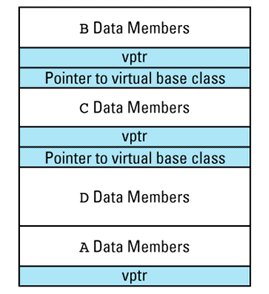
\includegraphics[keepaspectratio,width=0.2\paperwidth]{Pictures/mi-vptr.png}
	\caption{多重虚继承}
	\label{fig:mi-vptr}
	\end{center}
\end{figure}

就作用域而言,派生类作用域在基类作用域\textbf{之内}:查找名称时先查派生类。

一旦函数在基类中声明为虚函数,它就一直为虚函数,派生类无法改变该函数为虚函数这一事实。派生类重定义虚函数时,
可以使用 virtual 保留字,但不是必须这样做。

如果类的指针为空,用该指针可调用类的成员函数,编译不出错误。但如果成员函数为虚函数,或者访问了成员变量,会发生段错误。





\subsection{继承权限}


无论是公有继承还是私有继承,派生类对基类公/私有成员的访问权限\textbf{同用户代码完全一致},对\textbf{(本对象的)}基类保护成员的访问权限为真。

基类本身指定对自身成员的最小访问控制。派生类可以进一步\textbf{限制}(而非放松)对所继承的(private,protected)成员的访问:
\begin{itemize}
  \item 公有继承保留public,protected成员访问级别。struct默认公有继承。
  \item 保护继承将public,protected成员访问级别置为protected
  \item 私有继承将public,protected成员访问级别置为private。class默认private继承。
\end{itemize}
使用 private 或 protected 派生的类不继承基类的接口, 被称作通常被称为\textbf{实现继承(implemented-in-terms-of)}。
对于private继承,如果偶尔需要将个别基类成员置为public,可以在派生类定义式中使用\textbf{using语句声明一下该成员}就好。

派生类到基类转换的可访问性,取决于基类的public成员是否可访问。

组合的两个涵义分别是has-a和implemented-in-terms-of。对于implemented-in-terms-of,
优先选择组合而非私有继承,
除非当原始类(基类或被复合类)的protected成员和virtual函数被牵扯进来,
因为私有继承派生类可以冲定义virtual函数并访问protected成员,而复合对象却不可以。

友元关系不能被继承;构造、析构、拷贝构造、operator=不能被继承。



\subsection{new和delete}

调用new operator创建对象(\verb$new Widget;$)时,有两个函数被调用,一个是operator new,一个是对象的构造函数。
operator new至少接受一个整型参数,如果还接受一个指针参数,则被称作placement new。
placement new用于在已经分配好的原始内存上构建对象:\verb$new(buffer) Widget;$。


operator new无法满足分配需求时,不断调用new-handler,如果不存在new-handler会抛出\verb$bad_alloc$异常。老式的实现会返回null。

\subsection{对象构造控制}

C++可能为类自动创建\textbf{6种}函数:默认构造(\textbf{仅当别无构造函数时}),析构,赋值,拷贝构造,取址,const取址。
\textbf{这些函数只有它们真正被需要的时候才会被创建},作为public inline函数。

常用的构造控制技巧:
\begin{description}
\item[只允许单一实例]私有构造函数,返回static对象的公有接口
\item[禁止派生]私有构造函数,工厂接口。C++11 支持final关键词。
\item[禁止派生但允许栈上创建]如果不允许使用C++11 支持final关键词,那么令该类继承一个拥有私有构造/析构函数的基类,并将本类设置为基类的友元类。
\item[允许特定数量的对象]定义计数类模板,被计数类对其特化,并对其私有继承(参More Effective C++)。
计数类拥有static计数变量,为每个特化参数(被计数类型)计数,而不是为所有被计数类计总和
\item[只允许产生于Heap上]注意到Stack上的对象会自动调用构造和析构函数,可令类的析构函数为private,
再定义一个公有的伪析构函数(函数名任选)供知情的用户调用,伪析构函数调用“delete this;”操作完成真正的析构。
如果需要支持继承,可将析构函数定义为protected。如果需要支持composition,则容器类只能包含这个类的指针,而不是这个类的对象。
\item[不允许产生于Heap上]将operator new/delete置为私有,或置为=delete(C++11)
\item[判断对象是否在Heap上]做不到。但是可以在每次在堆上构造对象时进行簿记
\end{description}


                            


























